% General comments / corrections:
% - be consistent in use of "B" vs "B molecules"
%
\section{Introduction}
\label{sec:Introduction}
% - carbon blacks instead of soot (materials focus)

%% Curved carbons are everywhere...
Curved carbons are found in many materials including porous carbons, glassy carbons, activated carbons~\cite{Harris2005new,Martin2019topology,Martin2019nanostructure} and soot particles~\cite{Martin2018flexo}. For example, high resolution transmission electron microscopy of energy-relevant carbon materials such as coke and soot shows that a significant proportion (63\% for young particles, 28-49\% for mature carbons) of the constituent molecules are curved~\cite{wang2017improved,zhong2018structural,Martin2018flexo}. 
%Curved carbon molecules have many different names including bowl-shaped compounds, buckybowls, $\pi$-bowls, and fullerene-like fragments. In this work we will refer to them as curved polycyclic aromatic hydrocarbons (cPAHs), since flat polycyclic aromatic hydrocarbons (fPAHs) will be used as a comparison.
%% Curvature is caused by, properties 
This curvature is predominantly caused by the presence of non-hexagonal rings, such as pentagons, within a hexagonal lattice~\cite{Martin2018polar}. The resulting molecules, known as curved polycyclic aromatic hydrocarbons (cPAHs), have steric and electronic properties not present in defect-free carbon materials containing hexagonal structures only (flat polycyclic aromatic hydrocarbons, fPAHs). In particular, the curvature redistributes electronic charge in the $\pi$-cloud and causes the molecules to possess a dipole moment due to the flexoelectric effect~\cite{Martin2017}. This allows curved molecules to interact in long-range electrostatic interactions not present in systems containing planar carbon molecules, while still retaining aromaticity and show considerable electron delocalisation~\cite{grabowsky2010electron,Dobrowolski2011aromatic}.

%% curved carbon applications...
These qualities cause the presence of curved aromatic molecules to influence material structure and properties. Curved molecules increase material porosity~\cite{Harris2005new} and facilitate stronger adsorbate-adsorbent interactions~\cite{Martin2017} which, combined with high polarisability and high surface area, provide enhanced adsorption important for applications such as carbon sequestration, gas storage, and separation~\cite{Scanlon2006investigation}. Curved aromatics also possess a combination of properties, including surface charge stabilisation, high charge mobility, significant dipole moment, and small band gap~\cite{Menon2019optical}, that make them excellent candidates for applications such as optoelectronic devices, organic semiconductors, liquid crystals, electrodes, imaging probes, and batteries~\cite{roch2017indenocorannulene}. For example, integrating corannulene inside insulating porous scaffolds allows electronic properties to be tuned and results in a 10,000-fold conductivity enhancement~\cite{rice2018stack}. Flame-formed carbon nanoparticles show quantum dot behaviour~\cite{liu2019flame}, which have shown great promise in bioimaging as well as photovoltaic and light emitting applications due to their tunability, biocompatibility, luminosity, and solubility~\cite{zhang2012graphene}.
% Good promise in electronics applications because of tunable optoelectronic properties~\cite{sanyal2014functional}
% suggested for sensors and molecular machines (10.1039/c6cp05841h)

Accurately describing and characterising the self-assembly and nanostructure of curved carbon materials is of interest to production processes since curvature is easily integrated even when unintended. This is crucial for understanding many ubiquitous materials, such as combustion-produced pollutants~\cite{Martin2018flexo}, interstellar medium~\cite{Lovas2005}, and graphite synthesis from mesophase pitch. In particular, the degree of molecular alignment to form columnar or stacked structures plays a significant role in the mechanical and electronic properties of materials, such as high electron transport characteristics desirable for organic electron devices~\cite{wang2015electronic} and the generation of graphisiting material. There is some evidence that the presence of curved molecules contributes to a low degree of molecular ordering in a material~\cite{zhong2018structural} and prevents graphitisation of carbonised material by disrupting the formation of the mesophase~\cite{abrahamson2018carbon}. 
% In addition to providing the understanding required to optimise the nanostructures for these applications, this provides insight into the natural processes and environments that generate nanoparticles containing polycyclic aromatic hydrocarbons
%
%Carbon materials have been fabricated for use as adsorbents, carriers, catalyst supports, electrodes, and other advanced applications (refs).  The performance of these materials can be directly improved/tuned for these applications by adjusting their physical properties - in particular their nanostructures.  It is therefore crucial to develop a detailed understanding of the molecular interactions involved to enhance the prediction and design of desired carbon nanostructures.

%% Previous work looking at cPAH interactions:	Homogeneous dimers; Pi-pi > pi-CH interactions, eclipsed > staggered.
Previous work on the structure and properties of polycyclic aromatic hydrocarbons has focused on fPAHs~\cite{Grancic2016,chen2014size,Rapacioli2005stacked,hernandez2017dynamics}, with less attention given to cPAHs. Electronic structure calculations show that there are significant interactions between nested concave-to-convex homogeneous cPAH dimers~\cite{sygula2009pi,Cabaleiro-Lago2018} and, as with fPAHs, cPAH interactions are dominated by $\pi$-$\pi$ dispersion interactions with weaker contributions from CH-$\pi$ electrostatic interactions. That being said, electrostatics are more significant for cPAH interactions compared to non-polar fPAHs due to their permanent dipole moments~\cite{Cabaleiro-Lago2018,janowski2011convex}.
Different degrees of curvature result in increased or decreased cPAH dimer strengths, depending on the interplay of geometry and electrostatic effects. Curvature is able to increase interaction strength by decreasing C-C distances for increased dispersion interactions~\cite{kennedy2012buckyplates} but very curved molecules can also experience increased steric hinderance~\cite{sygula2009pi,Martin2018polar} and increased exchange-repulsion which serve to destabilise the dimer~\cite{kennedy2012buckyplates,sygula2009pi}.

%% Previous work looking at cPAH interactions:	Bulk systems
X-ray crystallography and density functional theory calculations have shown that the crystal structure of cPAH systems are determined by an interplay of electrostatic and dispersive forces, but predicting the packed structure of cPAHs is not straightforward. A molecule's dipole moment and molecule bowl depth are identified as significant factors, but do not have clear threshold values that guarantee particular molecular arrangements~\cite{Filatov2010}. In addition, the size~\cite{wu2006aromatic,forkey1997crystallographic}, curvature~\cite{petrukhina2004hemibuckminsterfullerene,bronstein2002practical,sakurai2005structural}, rigidity~\cite{sygula1994bowl,wang2015electronic}, functionalisation~\cite{sanyal2014functional}, and atomic composition~\cite{imamura1999triphenyleno} of cPAHs are known to influence their ability to form columnar stacks in solid state. These systems often show large $\pi$-$\pi$ overlap and staggered stacked interactions to produce extended $\pi$ networks enhanced by CH-$\pi$ interactions.

%% Previous work looking at cPAH interactions:	Heterogeneous systems (dimers, etc)
Preliminary work of larger molecular systems suggests that the self-assembly of homogeneous cPAH clusters is significantly different from similarly sized fPAH clusters~\cite{bowal2019ion}, which may be due to the ability of polar cPAHs to engage in electrostatic interactions. Computational studies show that the binding energies between fPAHs of different sizes are weaker than those within a homogeneous system containing one molecule size~\cite{Rapacioli2005stacked}. This heterogeneity decreases the stability of a nanoparticle containing different molecule sizes and leads to a distinct partitioning in which the larger molecules formed the cluster core and the smaller molecules resided in the outer shell~\cite{bowal2018partitioning}. The extent to which this nanostructure is also seen within cPAH systems has not yet been investigated, but dimer calculations suggest that bowl complementarity may produce different behaviour by enhancing the stability of heterogeoneous cPAHs clusters~\cite{Cabaleiro-Lago2018}. Previous work has also characterised the first solvation shells of fPAHs around an alkali-metal ion~\cite{bartolomei2019aggregation,bowal2019ion,Chen2016a}, but this has not been well-explored for cPAHs, which would likely self-assemble differently due to their polarity. It is therefore of great interest to understand how the fundamental interaction differences in shape and binding behaviour between fPAHs and cPAHs may influence their self-assembly in homogeneous and heterogeneous nanoparticles. To date detailed studies of cPAHs have primarily included electronic structure calculations or crystal structure experiments, as described above, neither of which provide information about intermolecular dynamics and particle nanostructure.
Previous work looking at systems containing cPAHs and fPAHs show the effect of structure on porosity and adsorption~\cite{zhang2020molecular,demir2016adsorption}, but do not evaluate the system dynamics which are crucial to understand self-assembly and structural properties. In addition, most work does not include the flexoelectric effects so long-range dipole-dipole electrostatic interactions are not included.
%
%The structural properties of cPAH clusters are unknown and further molecular modelling studies are required to provide insight into the clustering behaviour of cPAHs - their size-dependent arrangements in both homogeneous and heterogeneous systems, interactions with planar PAHs, and assembly around ions. Understanding non-covalent interactions with and between curved carbon nanostructures has importance in many systems and great potential for numerous applications.
% Development requires understanding of self-assembly and dynamic nanostructure of curved aromatics

The purpose of this work is to explore the self-assembly and internal nanostructure of clusters containing cPAHs, with the aim of answering the following questions relevant to carbon scientists from a myriad of fields: \textit{What is the energy and structure of cPAH nanoparticle systems and how do these differ from systems containing fPAHs? What is the influence of particle size, molecule size and proportion, and presence of ions or fPAHs?}  We address these by extending a force field parameterised for cPAH systems and using it within molecular dynamics simulations to provide a detailed assessment of cPAH cluster self-assembly. This analysis provides insight into the molecule interactions and nanoparticle structure that are important for better understanding carbon nanomaterials relevant to applications such as batteries, adsorbents, and optoelectronics.

%%%%%%%%%%%%%% Other notes to perhaps include %%%%%%%%%%%%%
% Functionalisation allows stacking solid-state structure in corannulene systems (chemical nature and position of functional groups strongly affects the stacking geometry) which influence optoelectronic properties~\cite{sanyal2014functional,mack2007development}.
% "Properties of a matter are intrinsically dependent on the internal arrangement of molecules in the solid state. Therefore, knowledge of three-dimensional structure of the matter is a prerequisite for structure–property correlations and design of functional materials. Over the past century, X-ray crystallography has evolved as a method of choice for accurate determination of molecular structure at atomic resolution. The structural information obtained from crystallographic analysis paved the way for rapid development in electronic devices, mineralogy, geosciences, materials science, pharmaceuticals, etc."
%
\section{Methods}
\subsection{Systems} %% systems studied
To thoroughly evaluate the self-assembly of nanoparticles containing cPAHs, three different molecule types with different sizes and degrees of curvature are considered: a small fPAH containing seven hexagonal rings (coronene, \ce{C24H12}), the smallest cPAH which contains one central pentagonal ring with five surrounding hexagonal rings (corannulene, \ce{C20H10}), and a larger cPAH containing two embedded pentagonal rings based on HRTEM analysis of early soot nanoparticles~\cite{Martin2018flexo} (\ce{C42H14}), all shown in Figure~\ref{fig:clustersnapshots}. The notation $\text{X}_{\text{y}}$ is used to describe the clusters studied, where X values refer to the molecule types and y gives the number of each type of molecule within the cluster. The molecule species considered in this work are: corannulene (indicated as A), \ce{C42H14} (B), coronene (C), circumcoronene (fPAH \ce{C54H18}) (D), and potassium cation (K). For example, $\text{A}_{\text{50}}\text{B}_{\text{50}}$ indicates a cluster containing 100 molecules, made up of 50 corannulene and 50 \ce{C42H14} molecules.

The influence of particle size, molecule size, molecule curvature, molecule ratio, and ion interactions are evaluated by considering 17 different clusters. Homogeneous clusters containing 25, 50, 100, and 200 of A and clusters containing 25, 50, and 100 of B are studied to provide information across molecule and cluster sizes. A series of heterogeneous clusters each containing 40 molecules of different sizes and proportions (A and B in proportions of 30:10, 20:20 and 10:30 are studied) allows evaluation of heterogeneity effects. In addition, a heterogeneous cluster containing 50 A and 50 B addresses heterogeneous cluster size effects. Clusters containing 20 A and 20 C provide insight into the interactions between cPAHs and fPAHs, and clusters containing 40 A or B with one or two potassium cations allow investigation into the self-assembly of ion-containing clusters. Snapshot images of each cluster considered in this work are shown in Figure~\ref{fig:clustersnapshots}. We should note that in this work, the terms (nano)particle and cluster are effectively synonymous: a nanoparticle is a cluster of molecules.

\subsection{Force field development}
Before any simulations can be conducted, the suitability of an intermolecular potential must be thoroughly evaluated. The isoPAHAP potential is an all-atom isotropic intermolecular description developed for fPAHs~\cite{totton2010first}. It shows good agreement with high accuracy quantum calculations and has been used in dynamic and stochastic simulations of fPAH systems~\cite{Totton2012quantitative,bowal2019sphere,Grancic2016,Pascazio2017}. This potential uses fixed atom-centred charges, which are suitable for fPAHs where electrostatic interactions arise principally from the terminal groups. It is not able to capture local dipole moments located at strained internal carbon sites within cPAHs. Therefore we recently developed a new atomic potential for cPAHs, called the curPAHIP potential~\cite{bowal2019ion}. The curPAHIP potential models the increased polarity of cPAHs using a modified molecule description with off-site point charges located above the pentagonal carbon atoms and optimised potential parameters parameterised to SAPT(DFT) energies.

Previous work introducing the curPAHIP potential included the cPAH A only. In this work, we extend the molecular description to include the larger cPAH B and assess the suitability of the curPAHIP potential for the new systems. Following the parameterisation method developed for A in~\citet{bowal2019ion}, B is minimised and mass-less charges are added 0.052~nm above each of the pentagonal carbon atoms to match the calculated dipole moment of 5.28~D~\cite{Martin2018flexo}. The resulting atomic coordinates and charges of the minimised B monomer (as well as A) are provided in Supplementary Information section~\ref{sec:SImoleculedesc}.

The binding energies of cPAH dimers are calculated to assess the suitability of curPAHIP in describing systems containing larger cPAHs. Density functional theory (DFT) calculations are used to determine the geometry of cPAH monomers and geometries and energies of cPAH dimers using a methodology similar to that used by~\citet{Martin2018polar} (see Supplementary Information section~\ref{secSI:DFT} for details). Binding energies are shown for four dimers in Figure~\ref{fig:potentialDFTcurves}. The energy computed with the isoPAHAP potential is also included to highlight the behaviour of a potential, developed for fPAHs, that does not include the enhanced electrostatics and dispersion due to the flexoelectric effect and increased polarisability, respectively, and in all cases the isoPAHAP potential significantly underestimates the binding energy and overestimates the equilibrium dimer distance.
The curPAHIP potential agrees well with the DFT and SAPT(DFT) results for the A dimer, see Figure~\ref{fig:potentialDFTcurves}(a). This is expected since these \textit{ab~initio} values were used in the parameterisation of the curPAHIP potential~\cite{bowal2019ion}. 
Figure~\ref{fig:potentialDFTcurves}(b) shows that the curPAHIP potential can be extended to cPAH molecules larger than A, since there is good agreement (within 5\% of the dispersion-corrected DFT energies) for the larger B. In contrast, the isoPAHAP gives a minimum energy value that is 31\% smaller than the DFT calculations.
The energies of heterogeneous dimers, containing one A and one B, are also well captured by the curPAHIP potential, as seen in Figure~\ref{fig:potentialDFTcurves}(c) and (d). The repulsive branch of the curPAHIP potential is slightly shifted to smaller distances than the DFT values in some cases, which is acceptable since the repulsive branch has been shown to weakly influence PAH cluster formation with the interaction well depth playing the significant role~\cite{Pascazio2017}.

An understanding of the potential error in structural metrics calculated from molecule arrangements caused by the use of the curPAHIP potential can be obtained by comparing to the DFT results. As the molecules used in the parameterisation of the potential, the A dimer shows no significant deviation.  For dimers containing B, there is a slight overall shift of around 0.2~nm between the curPAHIP potential energies and those calculated by DFT, which provides an estimate of the error in the intermolecular spacings determined in simulations using the cPAH intermolecular potential.  

Figure~\ref{fig:potentialDFTcurves} focuses on sandwich type interactions between cPAH dimers and we find that good agreement is also seen for the weaker T-shaped dimer interactions. Importantly, we see that the A T-shaped dimer interaction in which the molecules interact at the concave surface is stronger (by about 10 kJ/mol) than the T-shaped interaction of fPAH C, likely due to the flexoelectric dipole interacting with the C-H rim.  This enhanced interaction allows T-shaped interactions to be energetically favoured over sandwich interactions when many corannulene molecules are considered, such as in a cluster or bulk system.  %An increased corannulene dimer energy is not seen for the T-shaped dimer in which the molecules interact at the convex surface, with an interaction energy similar to that of the coronene T-shaped dimer.
It is also worth stating that the nested dimer with the smaller A on the concave side of the larger B (Figure~\ref{fig:potentialDFTcurves}(c)) shows a T-shaped type configuration. In this system the curPAHIP potential provides a slightly smaller angle between the two molecules in the minimum energy configuration than the DFT calculation, suggesting that CH-$\pi$ interactions are weaker and $\pi$-$\pi$ overlap is favoured using the intermolecular potential.  This difference does not seem to cause a significant difference in larger systems, however, as discussed further in the alignment angle analysis. 
%
\begin{figure}[!tbh]
\centering
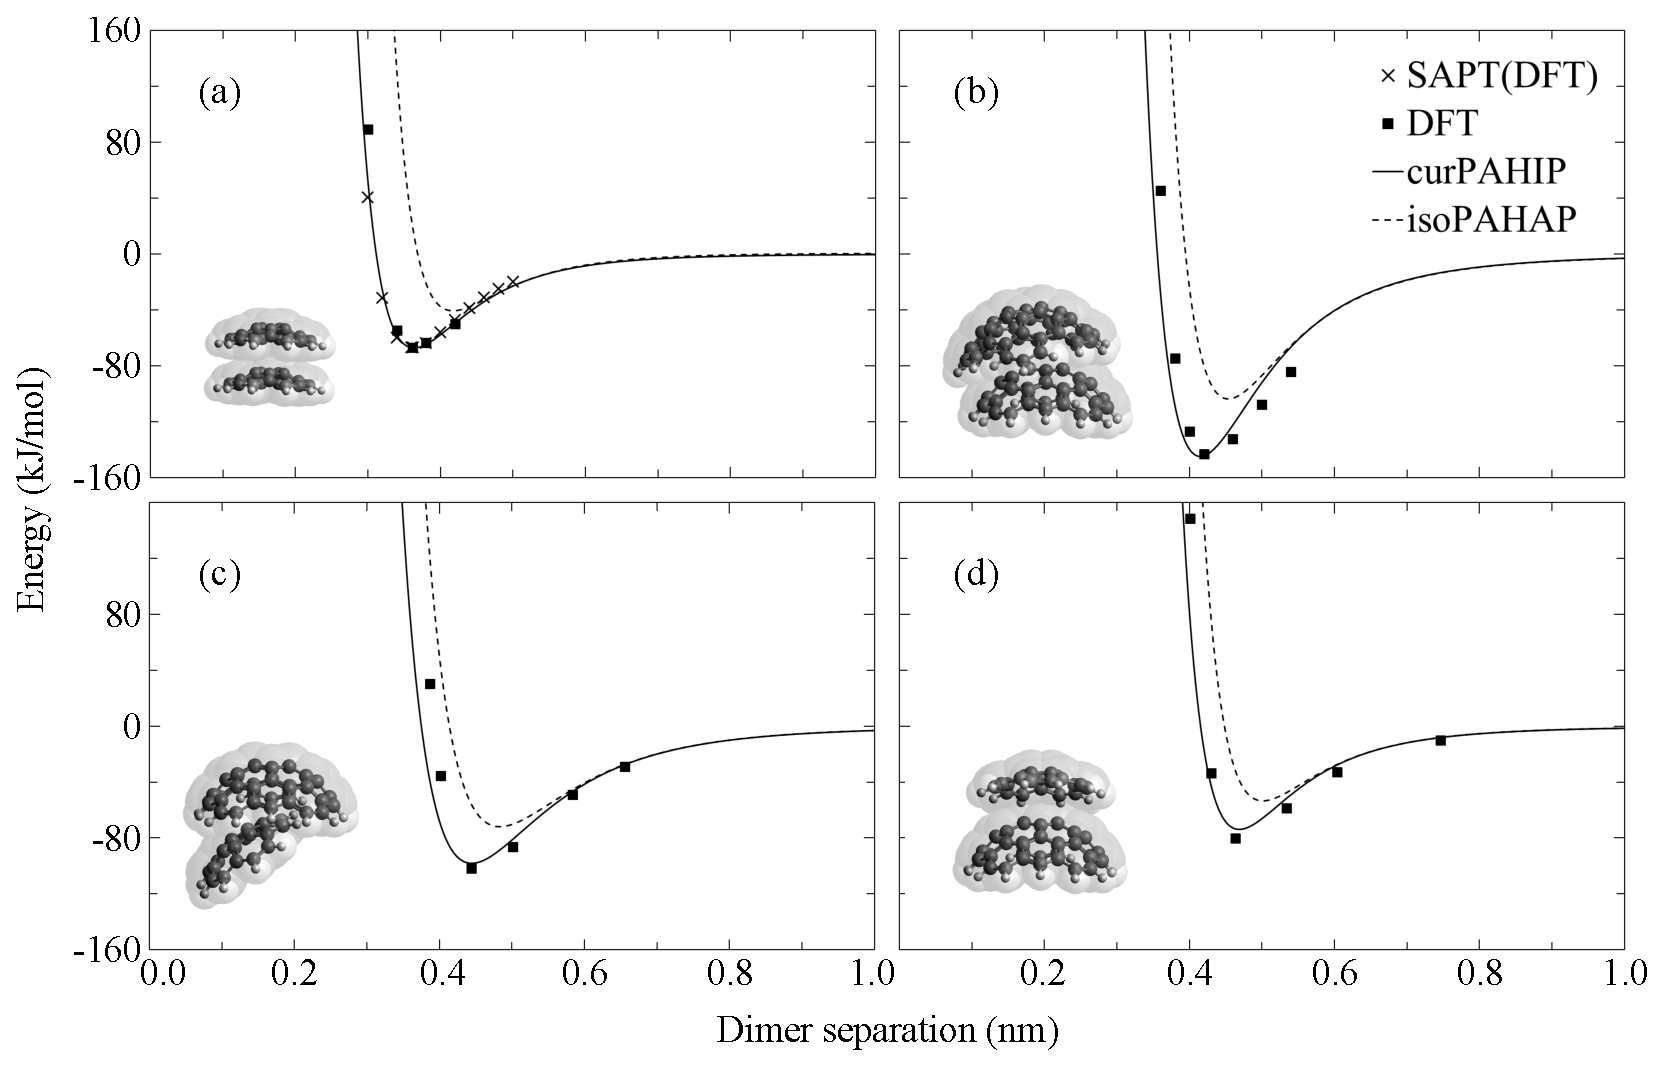
\includegraphics[width=1\linewidth]{Figures/potentialDFT_curves.eps}
\caption{Interaction energy versus separation distance for cPAH dimers determined from SAPT(DFT) calculations~\cite{Cabaleiro-Lago2018}, DFT calculations, the curPAHIP potential, and the isoPAHAP potential. The dimers are as follows: (a) two A, (b) two B, (c) and (d) one A and one B each.}
\label{fig:potentialDFTcurves}
\end{figure}
%

Further details on the isoPAHAP and curPAHIP potential form and parameters are found in Supplementary Information section~\ref{sec:SIpotentials}. For simulations considering both fPAHs and cPAHs in a single cluster, the curPAHIP potential was used to describe the mixed molecule interactions and simulations. Using the isoPAHAP potential to describe these interactions showed very similar results.

%%%%%%%%% perhaps to add to discussion:
% Overall some slight differences compared to DFT results show repulsive component of curPAHIP is shifted to smaller distances (means that there might be stronger attractions at small dimer separation distances) and minimum is slightly lower energy (provides conservative case if any different (less likely to bond))
% The difference between the DFT and curPAHIP energies can be partly explained by the fact that the MD minimised monomers (used in curPAHIP assessment) are more curved than the DFT monomers. So perhaps the energies are not as low for the curPAHIP potential since the dimers are not able to reach the same small distance values without steric hindrance and repulsion coming into effect.

\subsection{Molecular dynamics}
Equilibrium cluster configurations are produced using a multi-step molecular dynamics simulation process. Clusters are initialised in a mixed configuration, with molecules randomly placed within a large spherical volume using the PACKMOL software~\cite{Martinez2009PACKMOL}. Excess energy is removed by an energy minimisation step using the steepest descent algorithm, followed by the low-memory Broyden-Fletcher-Goldfarb-Shanno method~\cite{L-BFGS}.

Replica Exchange Molecular Dynamics (REMD) simulations are used to rapidly produce equilibrated cluster systems. Modelled after Monte Carlo parallel tempering~\cite{Hukushima1996}, REMD is an advanced form of molecular dynamics that involves evaluating simultaneous isothermal systems, called replicas, across a temperature range~\cite{Sugita1999}. At regular intervals throughout the simulation, neighbouring replicas are able to exchange spatial information based on a Boltzmann-weighted temperature dependent probability. This method allows efficient sampling of the system potential energy since low energy replicas are able to explore new configurations generated by higher energy replicas. 
% REMD simulations use a large number of interacting parallel simulations to rapidly determine stable structures across a large range of temperatures.
% able to rapidly determine low energy configurations by using higher energy parallel systems to explore new arrangements. % REMD was developed to enhance sampling of a complex potential energy surface, based on the fact that the rate at which barrier-crossing events occur is increased with an increase in temperature. 
% As a result, after an exchange, each low energy configuration exchanged into a higher energy replica has a better opportunity to overcome energy barriers and move into a new lower energy region of phase space, while each swapped high energy configuration provides a low energy replica with a fresh configuration to sample. 

In this work, REMD simulations are conducted for 3~ns. A large temperature range is selected to include solid-like and liquid-like particle morphologies. For clusters containing A, B, A and B, and A and C this corresponds to temperature ranges of 200--800~K, 400--1600~K, 200--1600~K, 200--800~K, respectively. These require between 27 and 84 REMD replicas to maintain an acceptable replica exchange acceptance. Further information detailing the replica temperature selection and an assessment of effectiveness is given in Supplementary Information section~\ref{secSI:REMDtemps}. As described in detail in similar work~\cite{bowal2018partitioning}, a flat-bottomed spherical position potential is applied within the REMD simulations to address complete evaporation of small molecules from the cluster at high temperatures. Individual 1~ns simulations using classical molecular dynamics (MD) are then conducted at each desired temperature from the final REMD configurations. No position potential is implemented for these post-REMD MD simulations.

In the REMD and MD simulations the NVT ensemble, where a constant number of atoms, system volume, and temperature are maintained, is sampled using chain of $10$~Nos\'{e}-Hoover thermostats for temperature control. A velocity Verlet integrator~\cite{Verlet_1967} is used to advance the configuration in 1~fs time steps and all simulations are conducted \textit{in vacuo} without periodic boundary conditions.  Intramolecular forces are determined using the OPLS-AA force field~\cite{Kaminski2001opls} for molecular bonds, angles, dihedral and improper dihedral angles. The curPAHIP intermolecular potential~\cite{bowal2019ion} is used to describe interactions between cPAHs and intermolecular cut-offs are set to $3.0$~nm. All minimisation, REMD, and MD simulations are conducted using GROMACS~5.1.4~\cite{Abraham2015}. Purpose-made scripts are used to the process the output and VMD~\cite{Humphrey1996} provides visualisations.


%%%%% Analyses %%%%%
\subsection{Structural analyses}
% Structural analysis - Molecular arrangement analysis (radial distances, coordination numbers, stacking angle, etc).
A number of different metrics, including density, intermolecular spacing, coordination number, alignment angle, and radial distance, are used to evaluate system structural properties. All metrics are averaged over the final 500~ps of the post-REMD MD simulation of the lowest temperature replica (\textit{i}.\textit{e}. 3.5--4.0~ns of total simulation time) using a timestep of 1~ps. 
%The final 500 ps of the post-REMD MD simulations are equilibrated and show <5\% drift in energy so this was selected as the production period.
Many calculations require the identification of near neighbours for each molecule within the system. For this, molecules are considered neighbouring if their centres of mass are within the cut-off radius $R$ for at least half of the 500~ps production period. Unless otherwise stated, values of $R$ are selected to allow $>85\%$ of molecules to have at least one identified neighbour. This results in cut-off radii of $R_{\text{A}} = 0.7$~nm, $R_{\text{B}} = 0.5$~nm, and $R_{\text{C}} = 0.5$~nm for A, B, and C, respectively.  The sensitivity of the cut-off values on calculated cluster properties is discussed in Supplementary Information section~\ref{secSI:cutoffs}.
% These cut-off radius values are used for both homogeneous and heterogeneous clusters 
%Although it may seem counter-intuitive that the smaller cPAH uses the larger cut-off distance, this is due to the different interaction types of the two molecules which will be discussed later.

%Intermolecular spacings are calculated between each molecule and its neighbours within $R$ and averaged over all equilibrated timesteps. The reported values are averaged over molecule type interactions in the system, including: all, B-B, A-A, and B-A.
Diameter and density values are determined using the solvent-excluded surface of the cluster calculated using a rolling sphere algorithm~\cite{sanner1996reduced}, as in previous work of fPAH clusters~\cite{chen2020reactive,bowal2020surface}. This provides values that are more accurate than commonly used spherical approximations since they are directly calculated from the three-dimensional surfaces.
% alignment angles
Molecular alignment angles are calculated to provide information on the relative configurations of neighbouring molecules within the clusters studied. An alignment angle is defined as the angle between normal vectors to the central rings (for A this is the pentagonal ring and for B this is the central hexagonal ring) of the neighbouring cPAHs considered.  Supplementary Information Figure~\ref{figSI:corannulene_crystal} provides a schematic of the alignment angle between two neighbouring A.
% coordination numbers
A quantitative measure of the degree of stacking order in the molecular structures is provided through the use of coordination numbers (CNs), calculated as the number of near neighbours averaged over each molecule type. To consider only $\pi$-$\pi$ stacking interactions within this metric, values of $R$ are selected to include sandwich-type stacked interactions between molecules but exclude molecules more than one layer away. Equilibrium dimer distances provide the minimum $R$ values for each molecule type as $R_{\text{A}} = 0.4$ nm and $R_{\text{B}} = 0.5$~nm.
% radial distances
Radial distance is defined as the distance between a molecule type and the cluster centre averaged over all atoms and provides insight into the spatial partitioning of molecule types within a cluster, particularly useful for understanding the self-assembly of heterogeneous systems. Further information on the calculation of the radial distances and coordination numbers is provided in Supplementary Information section~\ref{secSI:raddist_CN_eqns}.

%These metrics were assessed and represent the A crystal structure well (see Supplementary Information Section~\ref{secSI:corannulenecrystal} for more details).

\section{Results and Discussion}
%
Figure~\ref{fig:clustersnapshots} shows all of the low energy cluster geometries and Table~\ref{table:maintable} provides a summary table containing the corresponding structural metrics. The discussion of these results will be structured around questions in material and combustion science including:
\begin{itemize}
\item \textbf{Do cPAHs self-assemble into an ordered phase?} cPAHs clusters are analysed to explore the impact curvature has on the development of an ordered mesophase. 
\item \textbf{What is the internal nanostructure of cPAH nanoparticles?} cPAH clusters are evaluated with additional metrics (densities, radial distances, and energetics) to explore properties particularly relevant to combustion-generated nanoparticle pollutants and nanoparticle synthesis.
\item \textbf{How do complex cPAH systems self-assemble?} Clusters containing cPAHs with fPAHs or ions are structurally and energetically analysed to provide insights into real-world systems such as janus nanoparticles, battery materials, and combustion-generated nanoparticles.
\end{itemize}
%
\begin{figure}[!tbph]
\centering
\includegraphics[width=0.9\linewidth]{Figures/cluster_snapshots.eps}
\caption{Visualisations of the corannulene molecule (A, coloured green), \ce{C42H14} molecule (B, coloured purple), coronene molecule (C, coloured orange) and potassium cation (K, coloured grey), and clusters studied in this work. Ion-containing clusters are shaded to emphasise the solvation shell surrounding the ion(s).}
\label{fig:clustersnapshots}
\end{figure}
%
% TO DO: Reorder the table so columns match the order of discussion?
\begin{table}[ht]
\centering
\caption{Cluster diameter (nm), density (g/$cm^3$), intermolecular energy (kJ/mol per molecule), average intermolecular spacing (nm), average coordination number, and equilibrium radial distance, $r$, of molecule A and molecule B (nm) for all clusters studied in this work.} %Properties are empirical equilibrium values, as indicated by angled braces, determined as the average over the final 3~ns of the simulation.
\label{table:maintable}
\begin{tabular}{lccccccc}
\hline
\multicolumn{1}{l}{\multirow{2}{*}{Cluster}} & \multicolumn{1}{c}{\multirow{2}{*}{Diameter}} & \multicolumn{1}{c}{\multirow{2}{*}{Density}} & \multicolumn{1}{c}{\multirow{2}{*}{Energy}} & \multicolumn{1}{c}{\multirow{2}{*}{Spacing}} &
\multicolumn{1}{c}{\multirow{2}{*}{CN}} &\multicolumn{1}{c}{\multirow{2}{*}{$r_{\text{A}}$}} & 
\multicolumn{1}{c}{\multirow{2}{*}{$r_{\text{B}}$}} \\ 
\multicolumn{1}{c}{} & \multicolumn{1}{c}{} & \multicolumn{1}{c}{} & \multicolumn{1}{c}{} & \multicolumn{1}{c}{} & \multicolumn{1}{c}{} & \multicolumn{1}{c}{} \\ \hline
$\text{A}_{\text{25}}$ & 2.36 & 1.50 & -75 & 0.59 & 0.01 &  0.91 & -- \\
$\text{A}_{\text{40}}$ & 2.77 & 1.49 & -82 & 0.59 & 0.02 & 1.07 & -- \\
$\text{A}_{\text{50}}$ & 3.00 & 1.47 & -84 & 0.60 & 0.01 & 1.14 & -- \\
$\text{A}_{\text{100}}$ & 3.79 & 1.45 & -92 & 0.59 & 0.00 & 1.46 & -- \\
$\text{A}_{\text{200}}$ & 4.79 & 1.45 & -97 & 0.60 & 0.01 & 1.85 & -- \\ \hline
$\text{B}_{\text{25}}$ & 2.96 & 1.59 & -144 & 0.44 & 1.57 & -- & 1.27 \\
$\text{B}_{\text{40}}$ & 3.49 & 1.55 & -152 & 0.45 & 1.58 & -- & 1.45 \\
$\text{B}_{\text{50}}$ & 3.76 & 1.55 & -157 & 0.45 & 1.43 & -- & 1.49 \\
$\text{B}_{\text{100}}$ & 4.77 & 1.52 & -165 & 0.45 & 1.36 & -- & 1.92 \\ \hline
$\text{A}_{\text{10}}\text{B}_{\text{30}}$ & 3.31 & 1.58 & -147 & 0.44 & 1.04 & 1.53 & 1.30 \\ 
$\text{A}_{\text{20}}\text{B}_{\text{20}}$ & 3.16 & 1.55 & -125 & 0.44 & 0.92 & 1.31 & 1.20 \\
$\text{A}_{\text{50}}\text{B}_{\text{50}}$ & 4.31 & 1.52 & -135 & 0.51 & 0.70 & 1.85 & 1.49 \\ 
$\text{A}_{\text{30}}\text{B}_{\text{10}}$ & 2.98 & 1.52 & -103 & 0.54 & 0.74 & 1.21 & 1.04 \\ \hline
$\text{A}_{\text{20}}\text{C}_{\text{20}}$ & 2.88 & 1.46 & -80 & 0.43 & 0.74 & 1.18 & 1.21 ($r_{\text{C}}$) \\ \hline
$\text{A}_{\text{40}}\text{K}_{\text{1}}$ & 2.78 & 1.49 & -88 & 0.61 & 0.10 & 1.06 & -- \\
$\text{A}_{\text{40}}\text{K}_{\text{2}}$ & 2.79 & 1.48 & -94 & 0.58 & 0.20 & 1.05 & -- \\ 
$\text{B}_{\text{40}}\text{K}_{\text{1}}$ & 3.50 & 1.54 & -149 & 0.46 & 1.21 & -- & 1.35 \\ 
\end{tabular}
\end{table}
%

%%%%%%%%%%%%%%%%%%%%%%%%%%%%%%%%%%%%%%%%%%%%%%%%%%%%%
%%% Question 1: self-assemble to mesophase? %%%%%%%%%
%%%%%%%%%%%%%%%%%%%%%%%%%%%%%%%%%%%%%%%%%%%%%%%%%%%%%
\subsection{How do cPAHs self-assemble?} 
%How do cPAH self-assemble into a mesophase? 
As mentioned, mesophase formation (the molecular alignment of aromatic molecules) is critical for graphitisation. The intermolecular spacing, coordination number, and alignment angle values of molecules within homogeneous and heterogeneous clusters of cPAHs will be compared with similar clusters of fPAHs and experimental systems to provide insights into this question regarding cPAH self-assembly.

%% Intermolecular spacing: no cluster size dependence, suggests close interactions between large molecules (like dimer) compared to small molecules (which are more like crystal) %%%
Average intermolecular spacing is an important experimental quantity when tracking the formation of a mesophase and subsequent graphitisation as well as the presence of curvature in combustion carbons~\cite{botero2019internal}. The homogeneous cPAH clusters evaluated in this work have intermolecular spacings that do not change significantly with cluster size but depend strongly on the constituent molecule size. Clusters containing A possess an average intermolecular spacing of 0.59~nm while clusters containing B have an average spacing of 0.45~nm.  This shows that the spacings within homogeneous clusters are controlled by the molecular composition of the cluster rather than the number of molecules in a cluster.  Intuitively, one would expect the intermolecular spacing to increase with molecule curvature due to steric effects that prevent the molecules from interacting closely, however the opposite trend is observed.  This suggests that these two cPAH molecule types configure in different arrangements that are not controlled solely by steric effects.

To provide a comparison to reference molecule arrangements, the spacings of cPAH dimers using electronic structure calculations are (a) 0.36~nm, (b) 0.42~nm, (c), 0.44~nm, and (d) 0.46~nm, employing the same notation as in Figure~\ref{fig:potentialDFTcurves}. This shows that the average spacing of A within a homogeneous cluster is significantly larger than that of its sandwich dimer. The average intermolecular spacing within a single layer of the A crystal structure characterised by X-ray crystallography is 0.57~nm, suggesting the cluster structure of A likely possesses significant contributions from CH-$\pi$ interactions, in which the more positive region at the rim of one molecule is almost perpendicular to the negative region and the bottom of another molecule in a T-shaped configuration, rather than tight sandwich interactions. Further information on the A crystal structure is provided in Supplementary Information section~\ref{secSI:corannulenecrystal}. In contrast, the average intermolecular spacing of B cluster is similar to that of its sandwich dimer and similar to the spacing found in crystal structures of similarly curved indenocorannulene species (0.34--0.37~nm~\cite{Filatov2010}). The intermolecular spacings within clusters containing B do not change readily with the cut-off distance used, indicating that B have distinct near neighbours, for example in a highly stacked configuration. In contrast, A spacings are strongly correlated to the cut-off distance selected, suggesting that the molecules are not arranged in structured stacked layers. Intermolecular spacings are reported for a number of cut-off distances in Supplementary Information Table~\ref{tableSI:intermolecdistscutoff}.

The intermolecular spacings within heterogeneous cPAH clusters suggest that both the molecular ratio and cluster size play a role in the average spacing. This is investigated further in Table~\ref{table:mixedintermolecdists}, which breaks down the average results by considering the molecule type contributions to the intermolecular spacing. The interactions between molecules of the same type maintain spacings similar to those in the homogeneous clusters, so that the spacings between A are larger than those between B. As ion the homogeneous clusters, the B-B spacings are similar to that of a minimised B dimer and reasonably uniform across all heterogeneous clusters.  %slightly smaller than seen for B clusters
Cluster size does not influence the A-A spacing, however the proportion of A plays a role. The mixed molecule interactions have similar spacings to those of the larger cPAH suggesting that B promotes the close stacking behaviour of $\pi$-$\pi$ interactions with A. This is more pronounced in clusters with a higher proportion of B compared to A and is also cluster-size dependent. The differences between average spacings for the heterogeneous clusters (for example comparing $\text{A}_{\text{20}}\text{B}_{\text{20}}$ and $\text{A}_{\text{50}}\text{B}_{\text{50}}$) are therefore observed to be largely due to the number of neighbouring A or B within each cluster rather than the molecule type intermolecular spacings. % two50ann50 clusters show increased average spacings indicating stronger contributions from A-A interactions compared to B-B interactions, even compared to the two20ann20 clusters. %two20ann20 has 22 pairs for TWO-TWO and only 4 for ANN-ANN (and 21 for TWO-ANN); two50ann50 has 24 pairs for TWO-TWO and 26 for ANN-ANN (and 23 for TWO-ANN).
%In this way the cluster spacing averages provide an indication of which molecule neighbours are most prevalent.
This molecule type behaviour is likely due to the difference in curvature between these two cPAHs rather than the molecule sizes alone, since fPAH clusters containing a disparity of molecule sizes do not possess these differences (for example, a cluster containing 16 C and 16 D has an average spacing of 0.42~nm, with C-C spacings of 0.43~nm, C-D of 0.40~nm, and D-D of 0.41~nm~\cite{bowal2018partitioning}), 

%
\begin{table}[thb]
\centering
\caption{Intermolecular spacings within heterogeneous clusters, considering average distances between molecule types A and B.}
\label{table:mixedintermolecdists}
\begin{tabular}{lccc}
\hline
Cluster & B-B & B-A & A-A \\ \hline
$\text{A}_{\text{10}}\text{B}_{\text{30}}$ & 0.43 & 0.43 & 0.53 \\
$\text{A}_{\text{20}}\text{B}_{\text{20}}$ & 0.43 & 0.41 & 0.61 \\
$\text{A}_{\text{30}}\text{B}_{\text{10}}$ & 0.44 & 0.48 & 0.58 \\
$\text{A}_{\text{50}}\text{B}_{\text{50}}$ & 0.44 & 0.47 & 0.60 \\
\hline
\end{tabular}
\end{table}
% include proportion / percentage values for each interaction type from number of pairs in each case? 

%
These intermolecular spacings are significantly increased compared to planar carbons, especially for heterogeneous clusters. For example, a cluster containing fPAH 100~C~\cite{chen2014phase} has an average intermolecular spacing of 0.43~nm while all heterogeneous clusters have spacings $\geq$0.44~nm. In flame-produced soot particles similar spacings are found (0.38--0.48~nm depending on the particle maturity using high resolution transmission electron microscopy~\cite{botero2019internal,apicella2015soot}) to those seen for B and heterogeneous cPAH clusters. These results suggest that A or homogeneous clusters are not complete representations of these experimental systems and the intermolecular spacing is a useful quantity for detecting the presence of curvature in clusters and carbon materials. 
% It could also be interesting to explore how curvature influences mesophase formation and subsequent graphitisation to pristine graphite (with a spacing of 0.334~nm~\cite{Marsh2006}).

%%% CN results: 2pent15ring molecules are stacked, corannulene molecules aren't %%%
Coordination number values provide information on the extent of stacking interactions, which can help explain the intermolecular spacing results by identifying near neighbour patterns. In particular, this metric shows whether T-shaped interactions (in which molecules do not possess any near neighbours) or sandwich interactions (in which each molecule has one or two near neighbours) dominate. The homogeneous A clusters show an average CN of $0.01~\pm~0.01$, indicating predominantly T-shaped interactions, while the B clusters possess a CN of $1.48~\pm~0.09$, suggesting that they self-assemble with sandwich interactions. As seen in the cluster snapshots, B interact closely such that each molecule bowl inserts into the concave surface of its neighbour, allowing each molecule possesses on average more than one near neighbour in a stacked configuration. This is very similar to the arrangements of fPAH within clusters (for example, $\text{C}_{\text{100}}$ has an average CN of 1.6~\cite{chen2014size}) and cPAH hybrids that form tight stacks~\cite{dubceac2018self}. In contrast, A do not have near neighbours within stacking distance and the molecular bowls do not pack tightly within each other. As discussed by~\citet{liu2019flame}, molecular stacking is an important factor for the band gap of a PAH nanoparticle.
% add results from unit cell or other literature?

%%% CN results: addition of 2pent15ring into corannulene clusters increases stacking %%%
To further examine the influence of compositional heterogeneity, we compare CNs across different clusters each containing 40 cPAH molecules in Figure~\ref{fig:coordination_numbers}. The molecule-specific CNs within these heterogeneous clusters align with those calculated for homogeneous clusters. The B within all clusters have CNs above 1, indicating that on average these molecules have more than one near neighbour in a stacked arrangement. In contrast, all A have CNs significantly below 1, which shows that these molecules do not arrange in close stacks.  This suggests that the formation of an ordered phase is more likely with larger cPAHs compared to small species such as A. 
This molecule type difference, where smaller molecules possess lower CNs than larger molecules within a cluster, is also seen in fPAHs (for example, CNs of 2.00 and 1.25 for the C and D, respectively, within a $\text{C}_{\text{16}}\text{D}_{\text{16}}$ cluster) and is linked to the presence of smaller PAHs on the cluster surface (often by capping the ends of molecule stacks) compared to the bulk-residing larger PAHs.
% For these 40 molecule clusters, the CNs are: ann < 10t30a(a) < 2020(a) < 30t10a(a) < 10t30a(t) < 20/20(t)=two < 30t10a(t).  
The CNs for both cPAH sizes follow the trend $\text{A}_{\text{40}} < \text{A}_{\text{30}}\text{B}_{\text{10}} < \text{A}_{\text{20}}\text{B}_{\text{20}} < \text{A}_{\text{10}}\text{B}_{\text{30}}$ (shown with a solid arrow), illustrating that the addition of B into A clusters increases the degree of order and stacking.
%
\begin{figure}[!bth]
\centering
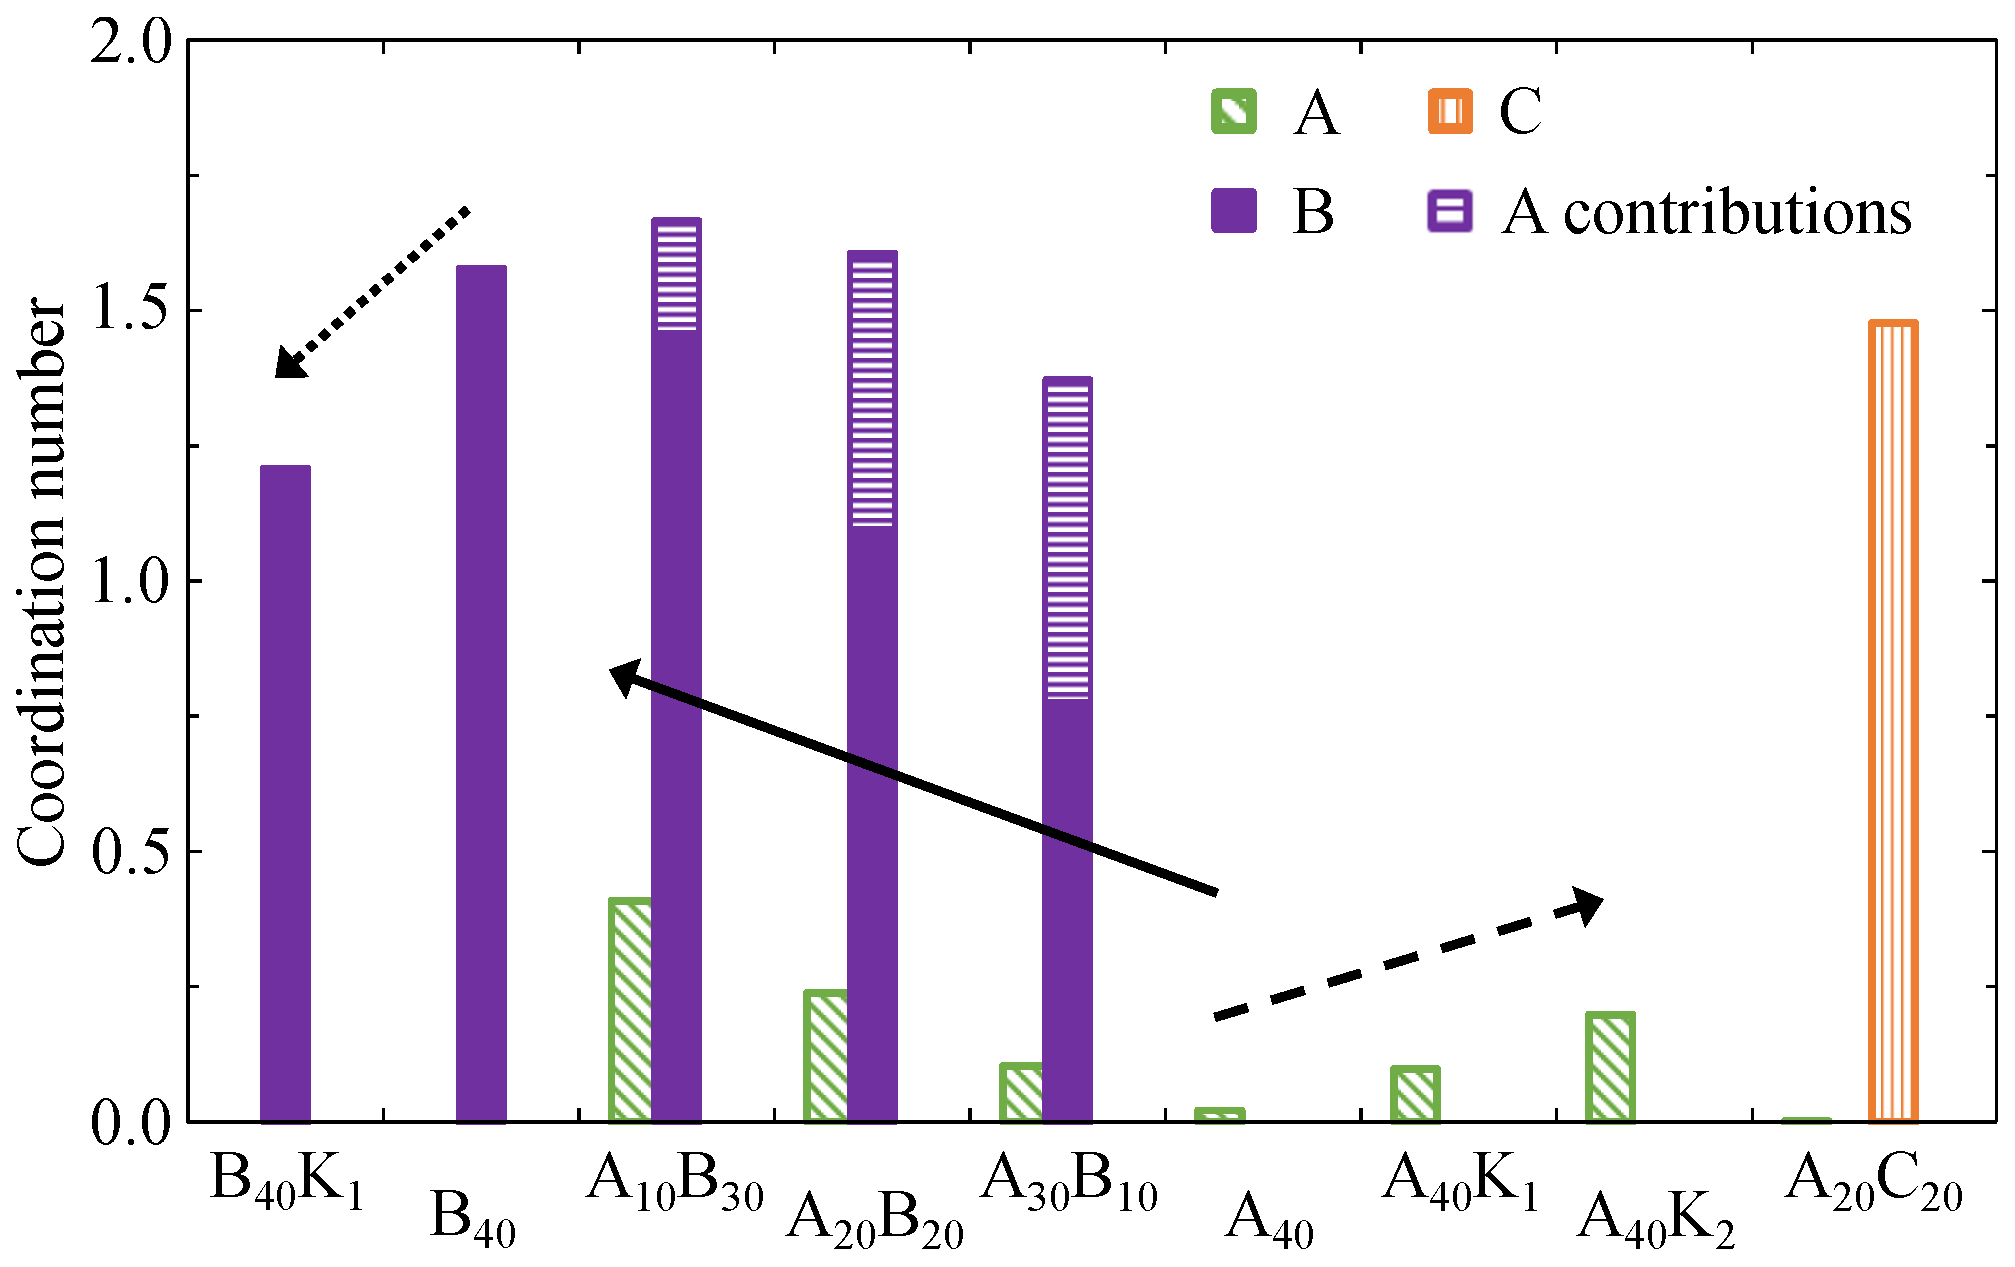
\includegraphics[width=0.8\linewidth]{Figures/CN_bar_chart_updated.eps}
\caption{molecule type coordination number values for clusters containing 40 PAHs.}
\label{fig:coordination_numbers}
\end{figure}
% perhaps include cluster snapshots with ribbons to show stacking more clearly?  As insets in bar chart?

We also are interested in which molecule types are present as near neighbours within these heterogeneous systems. We find that the CNs of A have no contribution from A, meaning that all A stacking interactions come from neighbouring B. The majority of B stacking interactions come from other B, however some of the interactions are with A in proportion to the molecular ratios within the cluster, shown as insets with horizontal lines in Fig \ref{fig:coordination_numbers}. This highlights that the smaller cPAH A interacts most strongly in the concave surface of the larger cPAH B, in agreement with calculated DFT dimer energies and our previous suggestion that interactions between bowl-complementing heterogeneous cPAH dimers could remove the strict steric constraints limiting the interaction strengths of homogeneous cPAHs~\cite{Martin2018polar}. 
% Contribution of B stacking that came from interactions with A are: two30ann10 12\%, two20ann20 32\%, two10ann30 43\%.

%%% Alignment angles: Molecule sizes have different angles %%% 
Figure~\ref{fig:alignmentangles_homo} presents histograms of the molecular alignment angles, illustrating the relative configurations of neighbouring molecules within the homogeneous clusters studied. It is again immediately clear that the two molecule sizes behave differently but these trends are consistent across all cluster sizes considered (additional cluster size plots can be seen in Figures \ref{fig:alignmentangles_hetero}, \ref{figSI:alignmentangles_cutoffs}, and \ref{figSI:alignmentangles_100}). The systems containing B (in the top row) show a single significant peak around 20$^{\circ}$.  This suggests that nearly all of the molecules interact in a tilted stack formation, forming one dimensional columns in which the molecule bowls possess a concave-to-convex alignment with dipole moment vectors nearly aligned. This small alignment angle provides significant $\pi$-$\pi$ overlap that, within columnar structures, is identified as a feature of materials with good performance in organic electronic devices. This dominant alignment angle is the same as that observed between a minimised B dimer (shown as a dashed vertical line), indicating that this is a stable arrangement.  Similar self-assembled structures are observed in crystals containing indenocorannulene molecules~\cite{Filatov2010} and other highly curved cPAHs that form polar crystals with strong photoluminescence~\cite{chen2014highly}. Neighbouring columnar stacks of B have opposite bowl directions and weak CH-$\pi$ interactions provide little interaction between columns. Interestingly, the columns show significant tilting at their ends such that parallel columns curve to be nearly continuous, which is not a feature of crystal structures and likely influences cluster surface properties. fPAH clusters, such as the representative $\text{C}_{\text{100}}$ shown in Figure~\ref{fig:alignmentangles_homo}, also show sharp angle peaks. However these peaks are centred around 0$^{\circ}$ and 180$^{\circ}$, which both correspond to aligned molecular planes (since the alignment angle calculation uses a normal vector). The variance in the fPAH alignment angles are likely from shifted interacting molecular planes as well as small tilting angles.
%% perhaps move the fPAH description to the beginning to highlight that B clusters are shifted?
This $\pi$-$\pi$ stacking arrangement combines with CH-$\pi$ interactions to produce a herringbone-like structure within both clusters and bulk crystal fPAHs~\cite{Khanna200567}, without the column curving present in cPAH clusters. 
% corannulene derivatives (with added rings) show significantly improved electrical conductivity compared to the parent corannulene~\cite{wang2015electronic} - suggests same for B

In contrast, clusters containing A (bottom row of Figure~\ref{fig:alignmentangles_homo}) show a dominant but broad peak around 45$^{\circ}$, with smaller wide peaks around 130$^{\circ}$ and 170$^{\circ}$. 
This agrees with previous work that shows A do not pack with any long-range order~\cite{hanson1976crystal,Petrukhina2005,kanao2018differentiating,wang2015electronic,scott1999geodesic} (the angles found in the crystal structure are shown as vertical dashed lines), with some CH-$\pi$ interactions but limited $\pi$-$\pi$ interactions. As seen in the dimer energies, the flexoelectric dipole enhances the interaction energy of T-shaped dimers in these small cPAHs so that, in contrast to the preferred stacked structure of fPAHs, this configuration becomes favoured for extended systems. It is interesting that this bulk molecular arrangement is observed even within the small nanocluster systems examined here. The method constraints of this work highlight that this structure is not due to the rapid bowl inversion dynamics or induced polarities within the system but instead to the molecule size, shape, and electrostatic properties.
% multidimensional analysis shows that the local orientational order of the corannulene molecules are more complex than those of 2pent15ring.  At smaller separation/cut-off distance (< XX nm), the favoured nearest neighbour geometry is XXX (like 45deg angled? vs stacked) while at larger distances (> XX nm) it is XXX (like 90deg??).

%
\begin{figure}[!tbh]
\centering
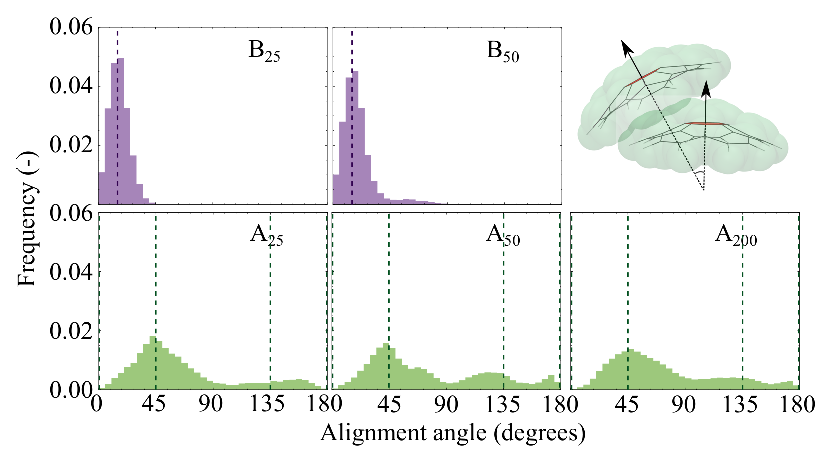
\includegraphics[width=0.84\linewidth]{Figures/alignment_angles_homo.eps}
\caption{Alignment angle distributions for homogeneous B and A clusters across different cluster sizes, with a fPAH cluster containing C included for comparison.}
\label{fig:alignmentangles_homo}
\end{figure}
%

Given that the two molecule types self-assemble with different alignment angles, we explore how mixing these molecules influences the alignment angle distributions. Figure~\ref{fig:alignmentangles_hetero} (second row) shows heterogeneous clusters each containing 40 molecules alongside the corresponding homogeneous clusters (third row). Additional results from larger clusters are found in Supplementary Information Figure~\ref{figSI:alignmentangles_100}. In all heterogeneous clusters, the individual molecule alignment peaks align reasonably well with those seen in the homogeneous clusters, A crystal structure, and B dimer, with the majority of B around 20$^{\circ}$ and many A around 45$^{\circ}$. There is an additional small B peak around 45$^{\circ}$, indicating some deviations from columnar stacking that align with the dominant arrangement of A. This is more pronounced in clusters containing $\geq$50\% A, suggesting that A molecules are located within B columns. The molecule proportions also influence A angles, with shifts towards lower angles and reduced values around 130$^{\circ}$. The $\text{A}_{\text{30}}\text{B}_{\text{10}}$ cluster shows a distribution similar to that of the homogeneous A cluster, although the peaks are much broader. As the proportion of B increases their influence is felt on A so that in the cluster containing equal ratios of both molecules ($\text{A}_{\text{20}}\text{B}_{\text{20}}$), the A peak at 45$^{\circ}$ is spread out towards 0$^{\circ}$ and the former 135$^{\circ}$ peak is pushed towards 170$^{\circ}$. In the cluster containing 75\% B ($\text{A}_{\text{10}}\text{B}_{\text{30}}$), the largest angle peak for A aligns with that of B at 20$^{\circ}$. This indicates that A are stacking in a similar fashion to B, which can be seen in the corresponding cluster snapshot (Figure~\ref{fig:clustersnapshots}) where A predominantly interact individually at the ends of B stacks, fitting in the concave or convex surfaces. Although similar molecule size interactions are observed in heterogeneous fPAH clusters, these planar aromatics do not self-assemble with different alignments depending on molecule size and thus heterogeneous clusters show the same highly aligned columnar stacking behaviour as homogeneous clusters, for example shown in the $\text{C}_{\text{16}}\text{D}_{\text{16}}$ cluster in Figure~\ref{fig:alignmentangles_hetero} (top row).
%
\begin{figure}[!tbh]
\centering
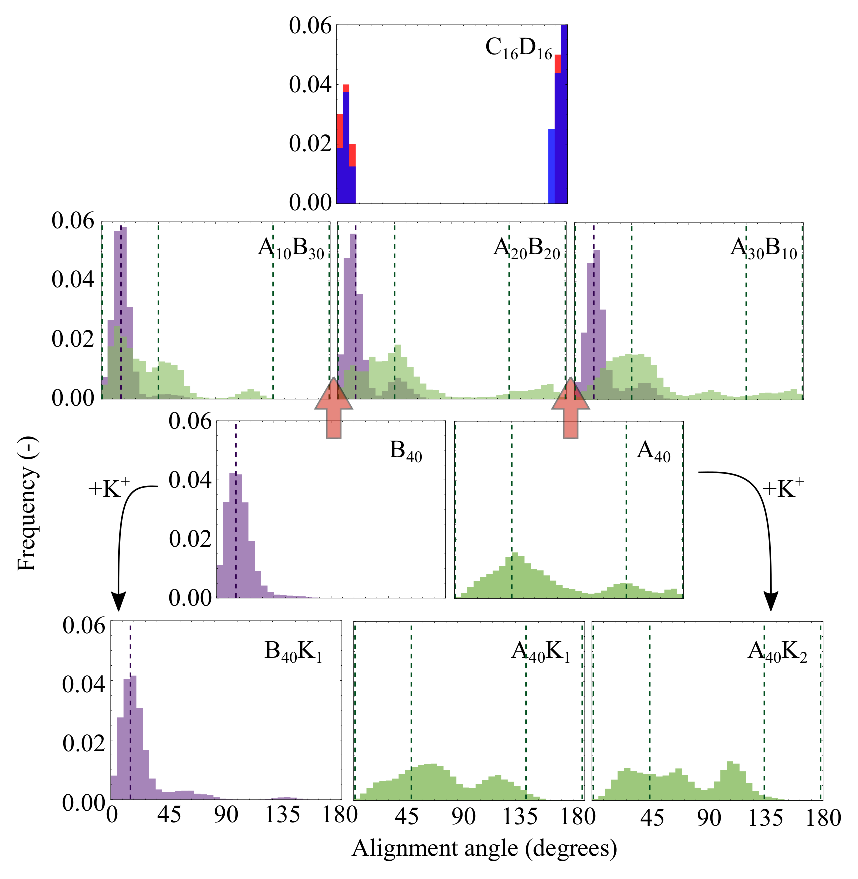
\includegraphics[width=0.85\linewidth]{Figures/alignment_angles_hetero.eps}
\caption{Alignment angle distributions for A and B clusters containing 40 molecules. The third row shows the homogeneous clusters, with red arrows showing the heterogeneous clusters (second row) and curved arrows indicating ion-containing clusters (bottom row). Angle distributions for a heterogeneous fPAH cluster (top row) obtained from~\citet{bowal2018partitioning} is provided for comparison.}
\label{fig:alignmentangles_hetero}
\end{figure}
%

This detailed evaluation of intermolecular spacing, CNs, and alignment angles shows that the self-assembly of cPAHs depends strongly on their molecular geometry and not the cluster size. Strong CH-$\pi$ attractions between molecule rims and bowl centres control the arrangement of A while dipole-dipole attractions and dispersion interactions control the nanostructure of B clusters. This molecule size dependent structure is observed within the crystal structures of cPAHs and also influences the behaviour of heterogeneous systems. Systems containing B show high CNs and low alignment angles, suggesting good molecular alignment similar to clusters of fPAHs. However, clusters containing even small proportions of A disrupt mesophase formation.
% curvature disrupts mesophase formation, particularly when mixtures of cPAHs are present.

% To add in somewhere?: Understanding the stacking behaviour of curved PAHs is relevant to materials studies / supramolecular chemistry / crystalline organic materials ( relevant to polymers of intrinsic microporosity, graphene systems, graphene quantum dots (experimental condensation structure)) because of their unique optical and conduction properties; and can also lead to using these molecules as building blocks for engineering organic crystals with desired properties.  

%%%%%%%%%%%%%%%%%%%%%%%%%%%%%%%%%%%%%%%%%%%%%%%%%%%%%
%%%% Question 2: What is the internal structure? %%%%
%%%%%%%%%%%%%%%%%%%%%%%%%%%%%%%%%%%%%%%%%%%%%%%%%%%%%
% Do cPAH self-assemble into core-shell nanoparticles?
\subsection{What is the internal structure of cPAH nanoparticles?}
Characterising the internal nanostructure of cPAH clusters provides valuable information relevant to the formation and composition of combustion-generated nanoparticles as well as the design of nanoparticles for optoelectronic applications. In this section we will discuss cluster densities and energies and will use radial distances to consider the partitioning behaviour of clusters containing different ratios of molecule sizes.

%% diameters and densities
Cluster diameters and densities show that cPAHs form tightly packed clusters. Homogeneous B clusters possess densities of 1.52--1.59 g/$\text{cm}^{3}$, which is comparable to mature graphitised soot particles (1.50--2.08 g/$\text{cm}^{3}$~\cite{johansson2017evolution}) although still lower than graphite (2.09--2.23~g/$\text{cm}^{3}$). Cluster densities for A are between 1.45 and 1.50~g/$\text{cm}^{3}$, higher than that of the A crystal structure (1.36~g/$\text{cm}^{3}$~\cite{Petrukhina2005}) and comparably sized fPAH clusters (1.39--1.46~g/$\text{cm}^{3}$~\cite{chen2014size}) but still within the range ascribed to young soot particles (1.12--1.50~g/$\text{cm}^{3}$~\cite{totton2010modelling,camacho2015mobility}). All cluster densities decrease with increasing cluster size, although this effect is muted for cPAH clusters compared to their fPAH counterparts. The diameter and density values of heterogeneous cPAH clusters are consistent with simple mixing averages of the analogous homogeneous cPAH clusters, suggesting that heterogeneity does not cause a dramatic change in the overall cluster shape and packing.

%%% Core-shell type partitioning of molecule sizes - not as distinct as fPAHs and not dependent on cluster size or molecular ratio %%%
We are particularly interested in whether cPAHs show the same core-shell partitioning seen in fPAH systems, where the cluster core consists of the larger fPAHs and the shell contains the smaller fPAHs~\cite{bowal2018partitioning}, which has been suggested to explain the core-shell nanostructure seen in combustion carbons. Average radial distances between each molecule type and the cluster centre are calculated to provide an indication of the molecule type positioning within each cluster, tabulated in  Table~\ref{table:maintable}. For the homogeneous cases, the two molecule types show similar relative average radial distances at 77--85\% of the total cluster radius, similar to the fPAH clusters (for example, $\text{C}_{\text{100}}$ has a value of 77\%~\cite{chen2014size}). However, in all clusters containing two molecule types A possess larger average radial distances (located within 80--90\% of the total cluster radius) than the B (70--80\% of the cluster radius). This is indicative of a core-shell structure in which the larger molecules reside in the cluster core, as seen in fPAH clusters (for example, the average radial distances of C and D are 89\% and 65\% of the cluster radius, respectively, for $\text{C}_{\text{16}}\text{D}_{\text{16}}$~\cite{bowal2018partitioning}). 

Although the average radial distances show a core-shell partitioning of molecule sizes, the equilibrium distribution of radial distances shows that this radial separation is less distinct for clusters containing cPAHs compared to similar fPAH clusters. Figure~\ref{fig:radialdists_atomic} shows that there is significant mixing of the molecule types within the cPAH clusters and molecules of both types are present near the cluster centre, regardless of cluster size or molecular ratio. This core-shell structure confirms that like fPAH clusters, cPAH clusters show the inverse molecular arrangement compared to that observed experimentally for mature combustion particulates~\cite{botero2019internal}, indicating that the core-shell nanostructure arises from carbonisation rather than physical partitioning of different sized PAHs.
%
\begin{figure}[!tbh]
\centering
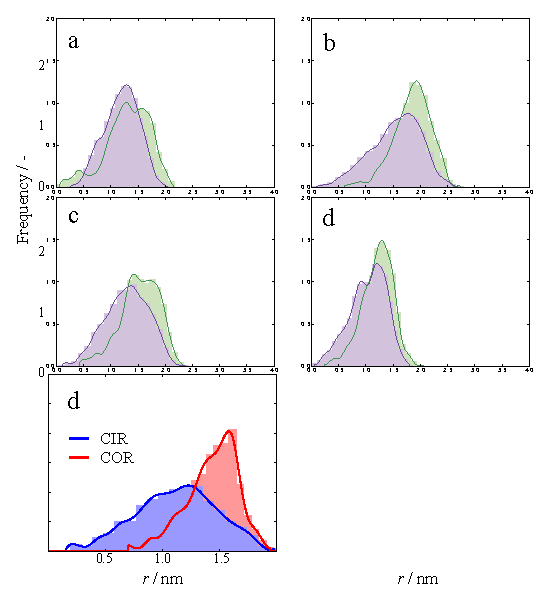
\includegraphics[width=0.6\linewidth]{Figures/radii_histograms_aa.eps}
\caption{Normalised atomic radial distance distributions for heterogeneous PAH clusters. The fPAH cluster $\text{C}_{\text{16}}\text{D}_{\text{16}}$ is obtained from~\citet{bowal2018partitioning}.}
\label{fig:radialdists_atomic}
\end{figure}
%

We previously explored the contribution of flexoelectrically polarised aromatics to soot formation~\cite{Martin2018flexo} and it follows that long-range dipole-dipole interactions between cPAHs may allow cPAH clusters to possess increased stability compared to fPAHs.  This would be of particular interest to contexts in which stable PAH nanoparticles are present, such as combustion and interstellar medium.  To address this hypothesis, we present intermolecular energies as a function of mass for cPAH and fPAH clusters, shown in Figure~\ref{fig:energies}.  The energies are shown per atom in the system in order to facilitate direct comparison between systems of different cluster and molecule sizes. It is clear that in all cases the energy decreases with cluster mass. Homogeneous clusters containing fPAHs (all coloured similarly here to allow for ease in reading), taken from~\citet{chen2014size,chen2015solid}, show relatively consistent energy trends across molecule sizes from pyrene to circumcoronene, with heterogeneous clusters, taken from~\citet{bowal2018partitioning}, generally at lower energies. Clusters containing cPAHs tend to have lower energies than fPAHs, as predicted based on their increased electrostatic attraction, although this is dependent on cPAH cluster composition. Clusters containing B show energies similar to those of heterogeneous fPAH clusters and A clusters possess lower mass-weighted energies. All cPAH clusters show significantly lower energies than the corresponding cPAH dimer interactions, which possess energies of $-0.93$--$-1.28$ kJ/mol atom. For reference, the experimental binding energy of graphite is $-2.4$--$-4.8$ kJ/mol atom~\cite{benedict1998microscopic}.

%
\begin{figure}[!tbh]
\centering
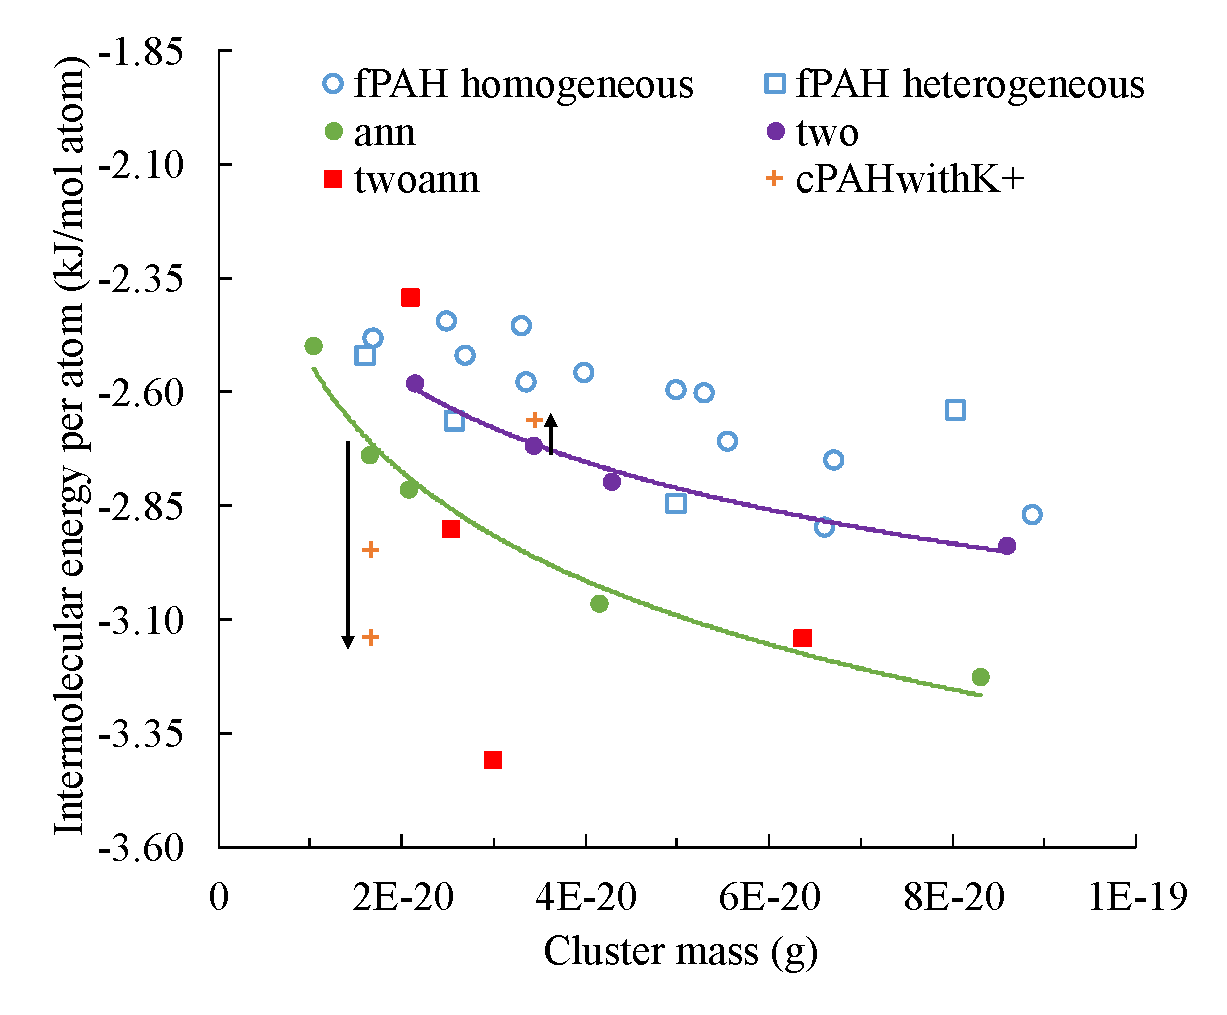
\includegraphics[width=0.8\linewidth]{Figures/energies.eps}
\caption{Intermolecular energy per atom versus cluster mass for all clusters considered in this work. Lines are drawn for the cPAH homogeneous clusters to guide the eye and black arrows show the energy changes caused by the addition of a cation(s). The subscript y is used to denote an unspecified number of molecules in order to consider multiple clusters. The experimental binding energy of graphite~\cite{benedict1998microscopic} is shown as a horizontal dashed line and possesses a large range from $-2.4$--$-4.8$ kJ/mol atom.}
\label{fig:energies}
\end{figure}

The effect of heterogeneity in cPAH clusters shows a distinct effect of molecular ratio: an increased proportion of B in the cluster decreases the energy. When there are equal numbers of both molecules, the heterogeneous cluster energies reflect those of homogeneous A clusters across cluster sizes. However, changing the molecule proportions affects the cluster energies significantly in that $\text{A}_{\text{30}}\text{B}_{\text{10}}$ possesses a high energy while $\text{A}_{\text{10}}\text{B}_{\text{30}}$ has a significantly low energy, producing the highest and lowest energy clusters of all the cPAH clusters evaluated. This suggests that in all cases the presence of B increases cluster stability if the composition is above 50\%.

These energy trends are in agreement with the structural metrics discussed previously, so that a higher degree of order within the hetergeneous cPAH clusters (increased stack formation as quantified by CNs, for example) corresponds to a greater interaction strength. This highlights that the stacking of A within the bowls of B increases the cluster intermolecular energy until a proportion (<50\% A) at which the presence of A disrupts B stacking by inserting within columns instead of only residing at column ends, thereby destabilising the cluster. %However, these enhancements are not sufficient to explain the rapid formation of soot nanoparticles in flames~\cite{Martin2018polar}. 
% TO DO: add summary statement to answer question

%%%%%%%%%%%%%%%%%%%%%%%%%%%%%%%%%%%%%%%%%%%%%%%%%%%%%
%%%% Section 3: complex cPAH clusters %%%%%%%%%%%%%%%
%%%%%%%%%%%%%%%%%%%%%%%%%%%%%%%%%%%%%%%%%%%%%%%%%%%%%
\subsection{How do complex cPAH systems self-assemble?}
Many practical applications involve systems that contain many molecule types. Of particular interest to combustion and material scientists are cPAH systems that also contain fPAHs or ions. We investigate relevant representative clusters using all of the metrics previously discussed to show the influence of different molecule curvatures and ion interactions within cPAH systems.

\subsubsection{Particles containing cPAHs and fPAHs}
To evaluate the self-assembly of clusters containing curved and flat PAHs, we consider $\text{A}_{\text{20}}\text{C}_{\text{20}}$. As seen in Figure~\ref{fig:clustersnapshots}, this cluster shows a distinct partitioning of the molecule types in a janus configuration, in contrast to the mixed arrangement seen in homogeneous clusters and the core-shell structure seen in heterogeneous clusters containing either fPAHs or cPAHs. The average intermolecular spacing of 0.43~nm (Figure~\ref{fig:coordination_numbers}) comes almost entirely from neighbouring C and matches the spacing calculated for a homogeneous C cluster~\cite{chen2014phase}. This suggests that the fPAH molecules orient in a stacked configuration, but the constituent cPAHs do not. This is highlighted in a detailed CN evaluation which shows constituent C have a CN of approximately 1.5 while A have no near neighbours within a stacked configuration cut-off radius (CN of 0.0). These structural values agree with the respective homogeneous C and A clusters, as do the molecular alignment angles (see Supplementary Information Figure~\ref{figSI:alignmentangles_ann20cor20}). The distinct types of local ordering cause the mixed fPAH and cPAH cluster to produce a janus particle with two different halves, highlighted by similar molecule type radial distances (see Table~\ref{table:maintable}). This cluster containing both curved and flat PAHs has an energy similar to that of homogeneous cPAH clusters, indicating that the mixing of molecule types does not enhance molecule interaction energy and instead it remains similar to that of the weaker component.

Dispersive and electrostatic interactions dominate the attractive forces between homogeneous interactions of fPAHs and cPAHs. However, this mixed molecule system is hindered by sterics and mismatched polarities and thus produces weaker interactions and a relatively low density. In this way the stronger interactions between like molecules contribute to a particle system in which the two molecule types are immiscible. Many material systems, such as coal and soot particles are seen experimentally to possess both curved and flat aromatics. These results suggest that when molecule type separation is not observed in such systems, self-assembly through physical interactions does not control the molecular structure. For example, covalent bonding between fPAHs and cPAHs may explain why soot particles do not form janus particles~\cite{Pascazio2019mechanical,Pascazio2020}.
%
%Relate these clusters and their properties to experimental structures (potential implications for synthesis, potential applications, etc).
% relevant to formation / nature of janus particles, for example ones that are polar on one side
% do not experience any enhancement in electrostatic interactions (in a non-polarisable potential description). not including some advanced interactions such as induced dipoles

\subsubsection{Particles containing cPAHs and ion(s)} 
%%% ions change the structure of cPAH clusters different depending on molecule size %%%
We further explore the influence of heterogeneity by considering clusters containing 40 molecules (A or B) and one or two potassium cations.  These systems can be directly compared to homogeneous systems of the same size. Potassium ions are selected because they are known to interact with cPAHs in systems of interest~\cite{Simonsson2017} and, importantly, because the intermolecular interactions between \ce{K+} and cPAHs have already been parameterised within the curPAHIP potential~\cite{bowal2019ion}. As seen in Table~\ref{table:maintable}, the inclusion of ion(s) within the cPAH clusters appears to increase the cluster diameter, and thus decrease the cluster density, slightly.

The cation(s) seems to have an effect on molecular arrangement that depends on the constituent cPAH size. The average CN of the B cluster decreases with the addition of \ce{K+} (shown by a dotted arrow in Figure~\ref{fig:coordination_numbers}), suggesting a disruption of the highly stacked ordering in agreement with an increased intermolecular spacing. Conversely, the A clusters show increased ordering with a higher CN (dashed arrow in Figure~\ref{fig:coordination_numbers}) and decreased spacing. This effect increases with the addition of a second cation suggesting that the cation influence is additive, although the CNs are still lower than those of the B clusters. %although further work needs to be done to assess when this trend reaches a saturation level or perhaps has cancelling or negative effects. 
The addition of a potassium cation(s) also results in decreased average radial distances for both molecule types, so that average molecular distance values are around 75\% of the total cluster radius.
In agreement with these structural metrics, the presence of cation(s) in the cluster has opposite effects on cluster energies: B clusters with \ce{K+} show an increased energy, while clusters with A containing \ce{K+} showed a decreased energy in proportion with the number of ions.  These differences are shown with black arrows in Figure~\ref{fig:energies}, again showing that the presence of an ion(s) influences molecular interactions and cluster structure in different ways depending on the molecule size.

The majority of B within an ion-containing cluster remain in tilted stacks with the alignment angle distribution, seen in Figure~\ref{fig:alignmentangles_hetero} (bottom row), showing a dominant peak at 20$^{\circ}$. Unlike the homogeneous B cluster, however, additional angles are present around 55$^{\circ}$ and 135$^{\circ}$. This shows that the addition of a cation causes some disruption to the stacked structure otherwise seen in homogeneous or heterogeneous clusters containing B. This is visible in the cluster image in Figure~\ref{fig:clustersnapshots}, which shows that the $\text{B}_{\text{40}}\text{K}_{\text{1}}$ possesses more short stacks compared to the long columnar structure of $\text{B}_{\text{40}}$.  The alignment angle distributions of A clusters containing \ce{K+} are significantly different than the homogeneous and heterogeneous cases as well as the crystal structure, with a broadening and splitting of the 45$^{\circ}$ peak, shift and increase of a peak around 110$^{\circ}$, and disappearance of high angles above 140$^{\circ}$.

These quantitative differences suggest that the addition of a cation promotes stacking within the A cluster and disrupts the existing stacking within the B cluster. This can be observed in the cluster visualisations in Figure~\ref{fig:clustersnapshots}, which highlight the atoms immediately around the cation(s). All clusters show a solvation shell of 4 molecules around each cation with the cPAH electron-rich convex surfaces face towards the cation(s). cPAHs form a tetrahedral-like formation, called a "flower`` motif in~\citet{bowal2019ion}, compared to the a staggered triangular "propeller`` motif adopted by fPAHs around a cation~\cite{bartolomei2019aggregation}. Steric effects allow this motif to serve as a seed for the A structure while disrupting the long stacks otherwise present in B clusters. This indicates that the self-assembly behaviour around cations depends on the cPAHs considered and so the addition of cations does not always increase molecular alignment and stability in large homogeneous clusters. These results also support the idea that a small cluster of 1--5 cPAH can be stabilised as an ionic nuclei that could contribute to other mechanisms for soot nanoparticle formation~\cite{Martin2018flexo}. 

\section{Conclusions}
Curved carbons are ubiquitous and have great promise in many systems and applications such as pollution reduction, novel nanocarbon materials, and sensors. This work provides a first detailed exploration of the self-assembly of particles containing cPAHs, examining their nanostructure in homogeneous clusters containing one molecule type only, heterogeneous clusters containing different cPAH sizes and ratios, and complexcPAH clusters containing fPAHs or cations.

We extended the previously developed curPAHIP potential to capture the interactions between large cPAHs and mixed cPAH systems and allow the simulations necessary for this analysis. Structural metrics, including intermolecular spacing, coordination number, and alignment angles show that the nanostructure of homogeneous cPAH particles is dependent on molecule size but unaffected by particle size (from 2--5~nm). B form parallel stacked columns whereas A do not possess short-range order, although both particle systems show similarities to the crystal structures of comparable cPAHs. Mixing of cPAH sizes influences particle structure. The addition of A to a particle containing B serves to enhance the $\pi$-$\pi$ stacking and interactions of A, resulting in lower energy particles. %Both the CN and energy values suggest that B clusters with some added (<50\%) A are the most stacked and stable.
Regardless of molecular ratio, heterogeneous cPAH particles show a core-shell type arrangement similar to the partitioning observed in fPAH particles but less distinct due to bowl complementarity. 

Particles containing fPAHs and cPAHs self-assemble into janus particles, with minimal interaction between the molecule types, suggesting that the two molecule types are not miscible. Further work to thoroughly develop a fPAH-cPAH intermolecular potential and test the effect of molecular composition should be done to further explore the formation and potential applications of semi-polar janus particles containing cPAHs and fPAHs. The addition of cations to cPAH particles causes the formation of a solvation shell that influences the internal particle structure. A show enhanced local order extending from the cation(s), while the stacked structure of B is disrupted due to the cation present. Further work should examine the influence of ion charge, size, and number on these structural properties. Future work should also consider the presence of additional atoms within cPAHs, since the interactions between curved aromatic molecules containing heteroatoms, such as oxygen, show increased dimer interactions that provide further electrostatic stabilisation~\cite{Cabaleiro-Lago2018}.  

\section*{Acknowledgements}
This work used the ARCHER UK National Supercomputing Service (\url{http://www.archer.ac.uk}).
K.B. is grateful to the Cambridge Trust and King's College, Cambridge for their financial support.
This project is also supported by the National Research Foundation (NRF), Prime Minister's Office, Singapore under its Campus for Research Excellence and Technological Enterprise (CREATE) programme.
